\documentclass{standalone}

\usepackage{tikz}
\usetikzlibrary{arrows}
\usetikzlibrary{decorations.markings}
\usepackage{standalone}

\begin{document}

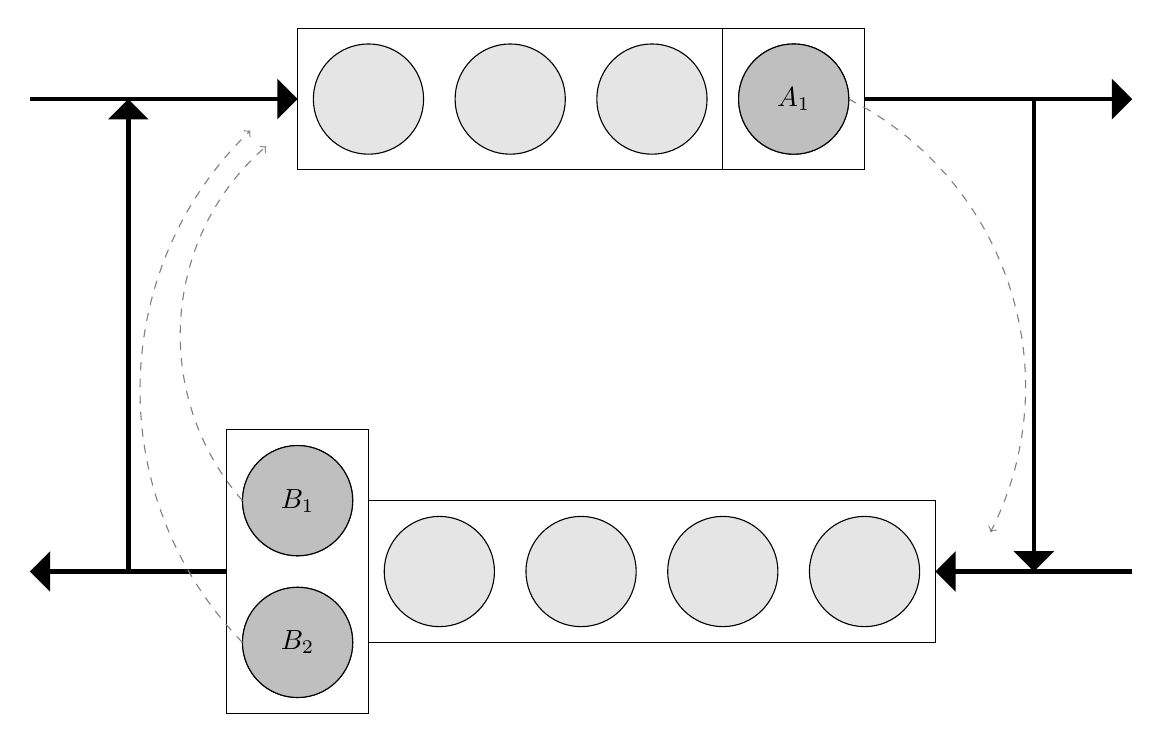
\begin{tikzpicture}


% Node middle
\draw (4.8, 8.1) rectangle (12, 9.9);
\draw (3, 7.2) rectangle (4.8, 10.8);

% Node top
\draw (3.9, 14.1) rectangle (9.3, 15.9);
\draw (9.3, 14.1) rectangle (11.1, 15.9);

% Routings
\draw[ultra thick, -triangle 90] (0.5, 15) -- (3.9, 15); % In to top
\draw[ultra thick, -triangle 90] (11.1, 15) -- (14.5, 15); % Out of top

\draw[ultra thick, -triangle 90] (14.5, 9) -- (12, 9); % In to top
\draw[ultra thick, -triangle 90] (3, 9) -- (0.5, 9); % Out of top

\draw[ultra thick, -triangle 90] (1.75, 9) -- (1.75, 15); % middle to top
\draw[ultra thick, -triangle 90] (13.25, 15) -- (13.25, 9); % top to middle

% Top customers
\node[align=center] [style={minimum size=1.4cm, text width=1.0cm, draw=black,fill=black!10,text=black,shape=circle}] at (10.2, 15) {$A_1$};
\node[align=center] [style={minimum size=1.4cm, text width=1.0cm, draw=black,fill=black!10,text=black,shape=circle}] at (4.8, 15) {};
\node[align=center] [style={minimum size=1.4cm, text width=1.0cm, draw=black,fill=black!10,text=black,shape=circle}] at (6.6, 15) {};
\node[align=center] [style={minimum size=1.4cm, text width=1.0cm, draw=black,fill=black!10,text=black,shape=circle}] at (8.4, 15) {};

% Bottom customers
\node[align=center] [style={minimum size=1.4cm, text width=1.0cm, draw=black,fill=black!10,text=black,shape=circle}] at (3.9, 9.9) {$B_1$};
\node[align=center] [style={minimum size=1.4cm, text width=1.0cm, draw=black,fill=black!10,text=black,shape=circle}] at (3.9, 8.1) {$B_2$};
\node[align=center] [style={minimum size=1.4cm, text width=1.0cm, draw=black,fill=black!10,text=black,shape=circle}] at (5.7, 9) {};
\node[align=center] [style={minimum size=1.4cm, text width=1.0cm, draw=black,fill=black!10,text=black,shape=circle}] at (7.5, 9) {};
\node[align=center] [style={minimum size=1.4cm, text width=1.0cm, draw=black,fill=black!10,text=black,shape=circle}] at (9.3, 9) {};
\node[align=center] [style={minimum size=1.4cm, text width=1.0cm, draw=black,fill=black!10,text=black,shape=circle}] at (11.1, 9) {};


\node[align=center] [style={minimum size=1.4cm, text width=1.0cm, draw=black,fill=black!25,text=black,shape=circle}] at (3.9, 9.9) {$B_1$};
\draw[gray, dashed, ->] (3.2, 9.9) [bend left=45] to (3.5, 14.4);

\node[align=center] [style={minimum size=1.4cm, text width=1.0cm, draw=black,fill=black!25,text=black,shape=circle}] at (10.2, 15) {$A_1$};
\draw[gray, dashed, ->] (10.9, 15) [bend left=45] to (12.7, 9.5);

\node[align=center] [style={minimum size=1.4cm, text width=1.0cm, draw=black,fill=black!25,text=black,shape=circle}] at (3.9, 8.1) {$B_2$};
\draw[gray, dashed, ->] (3.2, 8.1) [bend left=45] to (3.3, 14.6);

\end{tikzpicture}

\end{document}
